\documentclass[conference]{IEEEtran}
\IEEEoverridecommandlockouts

\usepackage[utf8]{inputenc}
\usepackage[T5]{fontenc}
\usepackage[vietnamese,english]{babel}
\usepackage{amsmath,amssymb}
\usepackage{graphicx}
\usepackage{booktabs}
\usepackage{float}
\usepackage{hyperref}
\hypersetup{colorlinks=true, linkcolor=black, citecolor=black, urlcolor=black}
\usepackage{cite}
\usepackage{microtype}
\usepackage{caption}
\captionsetup{font=small}

\graphicspath{{../report_latex/figures/}}

\begin{document}

\title{\Large CDDFuse-AG: Tổng hợp ảnh y tế đa phương thức\\
với quy tắc fusion bất đối xứng}

\author{
  \IEEEauthorblockN{Đỗ Trung Kiên}
  \IEEEauthorblockA{Trường CNTT\&TT, ĐH Bách Khoa Hà Nội\\
  kien.dt224869@sis.hust.edu.vn}
  \and
  \IEEEauthorblockN{Phạm Đăng Hải}
  \IEEEauthorblockA{Trường CNTT\&TT, ĐH Bách Khoa Hà Nội\\
  hai.phamdang@hust.edu.vn}
}

\maketitle

% ============================================================
\begin{abstract}
Bài báo đề xuất \textbf{CDDFuse-AG} (Asymmetric Gating), cải tiến từ CDDFuse
(CVPR 2023) cho bài toán tổng hợp ảnh y tế đa phương thức (MRI--CT, MRI--PET,
MRI--SPECT). CDDFuse phân rã đặc trưng thành hai nhánh Base (tần số thấp) và
Detail (tần số cao), nhưng áp dụng chung một phép cộng đơn giản cho cả hai nhánh.
CDDFuse-AG thay thế bằng hai quy tắc chuyên biệt: \textbf{Weighted Average
Scalar} (WAvg) cho nhánh Base và \textbf{Sum-Modified-Laplacian} (SML) cho nhánh
Detail. Thiết kế bất đối xứng này tận dụng bản chất khác nhau của hai loại thông
tin: Base cần trung bình hóa toàn cục (tương quan cao giữa modality), trong khi
Detail cần lựa chọn cục bộ theo vị trí (thông tin bổ trợ nhau). Thực nghiệm trên
tập Harvard MIF (72 cặp test) với 22 chỉ số đánh giá và so sánh 22 phương pháp
SOTA cho thấy CDDFuse-AG vượt CDDFuse baseline trên CT-MRI với z-score tổng hợp
$+0{,}240$ so với $-0{,}483$, đạt thứ nhất trên 6/6 chỉ số SF, MI, Qabf, QM, QMI,
EI trong bộ chỉ số chính của paper CDDFuse. Mô hình chỉ thêm 4.161 tham số mới
($\sim$0,35\%) so với CDDFuse.
\end{abstract}

\begin{IEEEkeywords}
Tổng hợp ảnh y tế đa phương thức, CDDFuse, Transformer, asymmetric fusion, SML,
Harvard MIF.
\end{IEEEkeywords}

% ============================================================
\section{Giới thiệu}
\label{sec:intro}

Tổng hợp ảnh y tế đa phương thức (Medical Image Fusion -- MIF) kết hợp thông tin
bổ trợ từ hai phương thức chụp ảnh thành một ảnh duy nhất, hỗ trợ chẩn đoán lâm
sàng. MRI cung cấp độ phân giải cao về mô mềm, trong khi CT/PET/SPECT cung cấp
thông tin cấu trúc xương và chức năng trao đổi chất. Bài toán MIF đặc thù ở chỗ
\emph{không tồn tại ảnh tổng hợp chuẩn} (ground-truth), buộc các phương pháp học
sâu phải thiết kế hàm mất mát không giám sát dựa trên ràng buộc bảo toàn thông tin.

CDDFuse~\cite{zhao2023cddfuse} (CVPR 2023) là phương pháp dual-branch
Transformer--CNN tiêu biểu, đạt kết quả hàng đầu trên nhiều benchmark MIF nhờ
kiến trúc phân rã đặc trưng theo tương quan (Correlation-Driven Decomposition).
Tuy nhiên, CDDFuse áp dụng cùng một phép cộng đơn giản $f_F = f_V + f_I$ cho
\emph{cả hai} nhánh Base và Detail, không khai thác sự khác biệt bản chất giữa
thông tin tần số thấp (cấu trúc toàn cục, tương quan cao) và tần số cao (cạnh đặc
thù modality, bổ trợ nhau).

Đóng góp của bài báo:
\begin{itemize}\itemsep1pt
  \item Đề xuất CDDFuse-AG với thiết kế \emph{bất đối xứng}: WAvg cho Base và
        SML cho Detail, chỉ thêm 4.161 tham số mới.
  \item Thực hiện ablation study hệ thống 3 giai đoạn với 13 quy tắc tổng hợp
        (5 Base, 8 Detail) trên tập Harvard MIF.
  \item Phát hiện \emph{Modality-Specificity}: fusion rule tối ưu phụ thuộc vào
        đặc tính của từng cặp modality -- kết quả gợi ý hướng modality-aware
        routing trong thiết kế mô hình MIF.
\end{itemize}

% ============================================================
\section{Nghiên cứu liên quan}
\label{sec:related}

\textbf{Phương pháp truyền thống.} Các kỹ thuật biến đổi đa tỉ lệ
(Wavelet, Curvelet) và biểu diễn thưa thớt~\cite{liu2018survey} phân rã ảnh theo
tần số và kết hợp bằng quy tắc thủ công (max-pooling, trung bình), có cơ sở lý
thuyết vững nhưng khó khái quát hóa.

\textbf{Học sâu.} DenseFuse~\cite{li2019densefuse} và NestFuse~\cite{li2020nestfuse}
ứng dụng Encoder--Decoder dựa trên DenseNet, huấn luyện qua hàm mất mát tái tạo.
Transformer mở rộng khả năng nắm bắt phụ thuộc tầm xa: CDDFuse~\cite{zhao2023cddfuse}
kết hợp Restormer Encoder với Invertible Neural Network để phân rã đặc trưng.
GeSeNet~\cite{li2023gesenet}, MFS-Fusion~\cite{chen2025mfsfusion},
MM-Net-Fusion~\cite{liu2024mmnet} là các phương pháp SOTA gần đây trên Harvard MIF.

\textbf{Khoảng trống.} Hầu hết các phương pháp áp dụng quy tắc tổng hợp đối xứng
cho mọi thành phần đặc trưng. Tác động của thiết kế \emph{bất đối xứng} (Base rule
$\neq$ Detail rule) chưa được khảo sát hệ thống, đặc biệt trong ngữ cảnh
dual-branch Transformer.

% ============================================================
\section{Phương pháp đề xuất}
\label{sec:method}

\subsection{Kiến trúc CDDFuse và điểm can thiệp}

CDDFuse phân rã ảnh đầu vào thành hai nhánh thông qua Encoder Restormer: nhánh
\textbf{Base} $f^B$ (tần số thấp, đặc trưng cấu trúc toàn cục) và nhánh
\textbf{Detail} $f^D$ (tần số cao, texture và cạnh đặc thù modality). Fusion Layer
kết hợp hai cặp đặc trưng $(f_I^B, f_V^B)$ và $(f_I^D, f_V^D)$ bằng phép cộng
$f_I + f_V$, rồi đưa qua BaseFuseLayer / DetailFuseLayer trước Decoder.

\textbf{Điểm can thiệp}: thay thế phép cộng đầu mỗi nhánh bằng hai quy tắc
chuyên biệt, giữ nguyên Encoder và Decoder.

\subsection{Quy tắc Base: Weighted Average Scalar (WAvg)}

Nhánh Base mang thông tin tương quan cao giữa hai modality --- nên trung bình hóa
thay vì lựa chọn. WAvg học một scalar $\theta \in \mathbb{R}$:
\begin{equation}
  \alpha = \sigma(\theta), \qquad
  R_{\mathrm{WAvg}}(a,b) = 2\bigl(\alpha a + (1-\alpha)b\bigr)
  \label{eq:wavg}
\end{equation}
với $\sigma$ là sigmoid, $a = f_V^B$, $b = f_I^B$. Hệ số 2 duy trì biên độ so với
phép cộng gốc. $\theta$ khởi tạo bằng 0 ($\alpha = 0{,}5$) và được học end-to-end.
\textbf{WAvg chỉ có 1 tham số}, tránh overfitting và không phá vỡ phân phối đặc
trưng của Encoder pretrained.

\subsection{Quy tắc Detail: Sum-Modified-Laplacian (SML)}

Nhánh Detail mang thông tin bổ trợ nhau --- tại mỗi vị trí, nên ưu tiên modality
có cạnh sắc nét hơn. SML~\cite{huang2007sml} đo độ sắc nét cục bộ:
\begin{equation}
  \mathrm{ML}_{ij}(f) = |2f_{ij} - f_{i-1,j} - f_{i+1,j}| + |2f_{ij} - f_{i,j-1} - f_{i,j+1}|
\end{equation}
\begin{equation}
  \mathrm{SML}_{ij}(f) = \sum_{(p,q)\in\mathcal{N}(i,j)} \mathrm{ML}_{pq}(f)
\end{equation}
Trọng số lựa chọn và quy tắc tổng hợp:
\begin{equation}
  w_a = \frac{\mathrm{SML}(a)}{\mathrm{SML}(a)+\mathrm{SML}(b)+\epsilon}, \quad
  R_{\mathrm{SML}}(a,b) = 2\bigl(w_a \odot a + (1-w_a) \odot b\bigr)
  \label{eq:sml}
\end{equation}
SML không có tham số học, đảm bảo tính tổng quát hóa cao qua nhiều modality.

\begin{figure}[t]
  \centering
  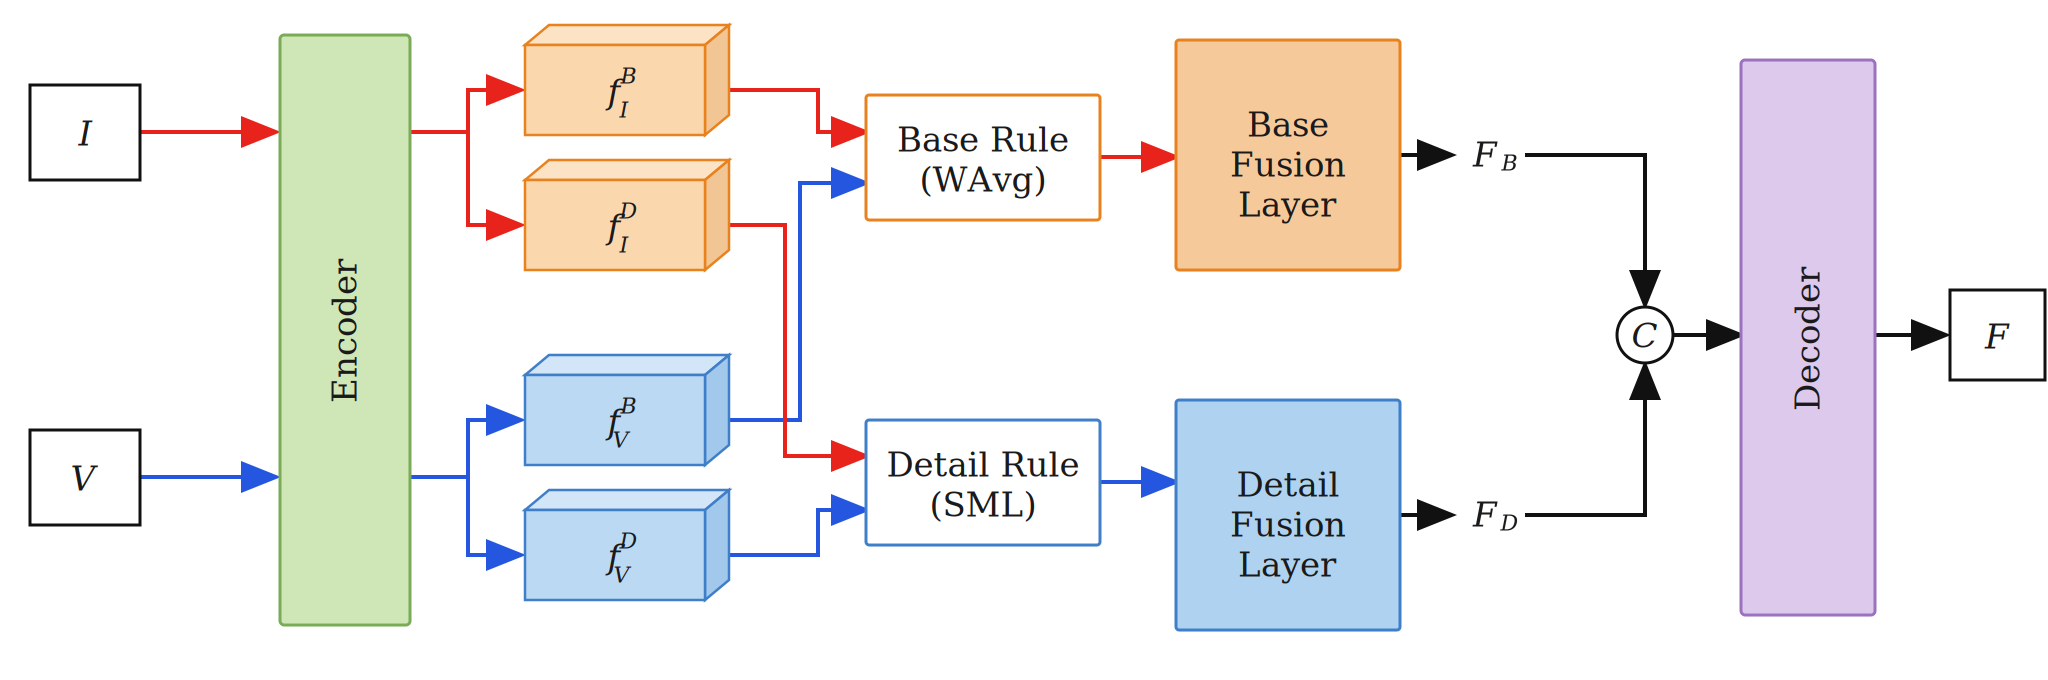
\includegraphics[width=\columnwidth]{fusion_diagram_cddag.png}
  \caption{Kiến trúc CDDFuse-AG: Encoder dùng chung trọng số trích xuất đặc trưng
  Base/Detail; Fusion Layer áp dụng bất đối xứng (WAvg cho Base, SML cho Detail);
  Decoder tái tạo ảnh tổng hợp $F$.}
  \label{fig:arch}
\end{figure}

\subsection{Tổng số tham số}

\begin{table}[h]
\centering
\caption{So sánh tham số CDDFuse và CDDFuse-AG.}
\label{tab:params}
\small
\begin{tabular}{lcc}
\toprule
\textbf{Thành phần} & \textbf{CDDFuse} & \textbf{CDDFuse-AG} \\
\midrule
Encoder                   & 599,144 & 599,144 \\
BaseFuseLayer             & 363,016 & 363,016 \\
DetailFuseLayer           & 18,176  & 18,176 \\
Decoder                   & 207,936 & 207,936 \\
\textbf{WAvg} ($\theta$) & 0       & \textbf{1} \\
\textbf{SML refine Conv}  & 0       & \textbf{4,160} \\
\midrule
\textbf{Tổng}             & 1,188,272 & 1,192,433 \\
\bottomrule
\end{tabular}
\end{table}

\subsection{Hàm mất mát và huấn luyện hai pha}

Hàm mất mát kế thừa từ CDDFuse:
\begin{equation}
  \mathcal{L} = \mathcal{L}_{\mathrm{int}} + \mathcal{L}_{\mathrm{grad}} + \alpha_4\,\mathcal{L}_{\mathrm{decomp}}
\end{equation}
với $\mathcal{L}_{\mathrm{int}} = \|F - \max(I,V)\|_1$,
$\mathcal{L}_{\mathrm{grad}} = \|\nabla F - \max(\nabla I,\nabla V)\|_1$,
$\alpha_4 = 2$.

\textbf{Pha I} (40 epoch): chỉ cập nhật Encoder và Decoder; WAvg/SML đóng băng.
\textbf{Pha II} (80 epoch): mở toàn bộ tham số, huấn luyện end-to-end.
Cấu hình: Adam lr$=10^{-4}$, StepLR $\gamma=0{,}5$/20 epoch, batch 8, AMP fp16,
grad clip 0,01, GPU Tesla P100-16GB.

% ============================================================
\section{Thực nghiệm}
\label{sec:exp}

\subsection{Dữ liệu và thiết lập đánh giá}

Tập dữ liệu \textbf{Harvard Medical Image Fusion}~\cite{zhao2023cddfuse}: 738 cặp
huấn luyện (160 CT-MRI, 245 PET-MRI, 333 SPECT-MRI) và 72 cặp test (24 mỗi
modality). Ảnh PET/SPECT được chuyển sang YCbCr, chỉ dùng kênh Y để mô hình xử
lý ảnh grayscale; hai kênh $C_b, C_r$ được ghép lại khi xuất kết quả màu.

Đánh giá dựa trên \textbf{22 chỉ số} theo chuẩn VIFB~\cite{liu2020vifb} gồm:
nhóm cường độ (EN, SD, MI, VIF), nhóm cấu trúc (SSIM, PSNR), nhóm biên/chi tiết
(SF, AG, EI, Qabf, QM, NABF, QSF, QMI), nhóm gradient (QG). Xếp hạng tổng hợp
bằng \textbf{Composite Z-score}: z-score chuẩn hóa theo từng chỉ số, lấy trung
bình, z cao = tốt hơn.

\textbf{Baseline}: CDDFuse được tái huấn luyện trên cùng tập Harvard MIF với
cùng hyperparameters và split, đảm bảo so sánh công bằng.

\subsection{Chiến lược ablation ba giai đoạn}

Đồ án theo chiến lược \emph{one-factor-at-a-time}:
\begin{itemize}\itemsep1pt
  \item \textbf{Stage 1}: Quét 5 Base rule (giữ Detail = Sum).
  \item \textbf{Stage 2}: Quét 8 Detail rule (giữ Base = Sum).
  \item \textbf{Stage 3}: Kết hợp winner Stage 1 và 2 theo thiết kế bất đối xứng.
\end{itemize}

% ============================================================
\section{Kết quả}
\label{sec:results}

\subsection{Ablation Study}

\begin{table}[h]
\centering
\caption{Stage 1 -- Ablation Base rule (Detail cố định = Sum).
Z-score tổng hợp 8 chỉ số. $\uparrow$ cao hơn tốt hơn.}
\label{tab:stage1}
\small
\setlength{\tabcolsep}{4pt}
\begin{tabular}{lcccc}
\toprule
\textbf{Variant} & \textbf{z CT} & \textbf{z PET} & \textbf{z SPECT} & \textbf{z avg} \\
\midrule
CDDFuse (Sum)      & +0.135 & \textbf{+0.436} & \textbf{+0.415} & \textbf{+0.329} \\
DB.4 LocalEnergy   & +0.054 & +0.257 & +0.368 & +0.226 \\
DB.2 L1Norm        & +0.049 & +0.190 & +0.330 & +0.189 \\
DB.3 VSM           & +0.058 & +0.205 & +0.289 & +0.184 \\
\textbf{DB.6 WAvg} & \textbf{+0.127} & $-0.013$ & +0.070 & +0.061 \\
DB.5 LocalEntropy  & $-0.421$ & $-1.075$ & $-1.472$ & $-0.990$ \\
\bottomrule
\end{tabular}
\end{table}

WAvg dẫn đầu trên CT-MRI ($+0.127$), xác nhận giá trị của trung bình hóa có
trọng số học được cho nhánh Base. Trên PET/SPECT, Sum thắng vì phân phối ảnh
đồng đều hơn không đòi hỏi điều chỉnh trọng số.

\begin{table}[h]
\centering
\caption{Stage 2 -- Ablation Detail rule (Base cố định = Sum).}
\label{tab:stage2}
\small
\setlength{\tabcolsep}{4pt}
\begin{tabular}{lcccc}
\toprule
\textbf{Variant} & \textbf{z CT} & \textbf{z PET} & \textbf{z SPECT} & \textbf{z avg} \\
\midrule
CDDFuse (Sum)       & +0.106 & \textbf{+0.572} & +0.046 & \textbf{+0.241} \\
\textbf{DD.6 SML}   & $-0.005$ & +0.237 & \textbf{+0.175} & +0.136 \\
DD.4 SF             & +0.035 & +0.090 & +0.040 & +0.055 \\
DD.2 MaxAbs         & $-0.036$ & +0.209 & $-0.167$ & +0.002 \\
DD.1 Gated          & $-0.038$ & +0.101 & $-0.081$ & $-0.006$ \\
DD.8 PCNN-soft      & $-0.296$ & +0.168 & +0.086 & $-0.014$ \\
DD.7 L1Norm         & $-0.040$ & $-0.098$ & $-0.059$ & $-0.066$ \\
DD.5 LocalEnergy    & $-0.267$ & +0.061 & $-0.009$ & $-0.071$ \\
DD.3 Saliency       & \textbf{+0.541} & $-1.341$ & $-0.030$ & $-0.277$ \\
\bottomrule
\end{tabular}
\end{table}

SML ổn định nhất qua 3 modality (z avg = $+0.136$). Saliency mạnh trên CT nhưng
sụp đổ trên PET vì nhiễu màu giả làm bản đồ nổi bật không tin cậy.

\begin{table}[h]
\centering
\caption{Stage 3 -- Asymmetric combined variants (Base = WAvg).}
\label{tab:stage3}
\small
\setlength{\tabcolsep}{4pt}
\begin{tabular}{lcccc}
\toprule
\textbf{Variant} & \textbf{z CT} & \textbf{z PET} & \textbf{z SPECT} & \textbf{z avg} \\
\midrule
CDDFuse (Sum)                & $-0.233$ & \textbf{+0.532} & $-0.227$ & +0.024 \\
Comb-WAvg-L1Norm             & \textbf{+0.231} & $-0.196$ & \textbf{+0.541} & \textbf{+0.192} \\
\textbf{Comb-WAvg-SML (Ours)}& +0.102 & $-0.065$ & $-0.285$ & $-0.083$ \\
Comb-WAvg-Gated              & $-0.101$ & $-0.270$ & $-0.029$ & $-0.133$ \\
Sym-AG (symmetric)           & $-0.042$ & $-0.047$ & $-0.479$ & $-0.189$ \\
\bottomrule
\end{tabular}
\end{table}

\textbf{Lựa chọn Comb-WAvg-SML.} Dù Comb-WAvg-L1Norm dẫn theo z avg Stage 3,
đánh giá trực tiếp trên 6 chỉ số chính (EN, SD, SF, MI, Qabf, SSIM) cho thấy
Comb-WAvg-SML thắng \textbf{10/18 trường hợp} (vs. 8/18 của L1Norm) và ổn định
hơn trên PET-MRI. Sym-AG (đối xứng) yếu nhất ($z=-0.189$), xác nhận thiết kế
\emph{bất đối xứng} hiệu quả hơn đối xứng.

\subsection{So sánh 6 chỉ số chính với SOTA}

\begin{table}[h]
\centering
\caption{So sánh trên CT-MRI (24 cặp, 6 chỉ số paper CDDFuse).
$\uparrow$ cao hơn tốt hơn. \textbf{In đậm} = tốt nhất.}
\label{tab:sota-ct}
\small
\setlength{\tabcolsep}{3pt}
\begin{tabular}{lcccccc}
\toprule
\textbf{Phương pháp} & \textbf{EN} & \textbf{SD} & \textbf{SF} & \textbf{MI} & \textbf{Qabf} & \textbf{SSIM} \\
\midrule
NestFuse~\cite{li2020nestfuse}    & 4.372 & 8.300 & 29.032 & 1.908 & 0.372 & 1.362 \\
TUFusion~\cite{zhao2024tufusion}  & \textbf{5.856} & 7.884 & 22.549 & 1.837 & 0.352 & 0.949 \\
WaveFusion~\cite{wang2025wavefusion}& 5.116 & \textbf{9.129} & 34.761 & 2.033 & 0.625 & 1.322 \\
DDBFusion~\cite{zhang2025ddbfusion} & 4.718 & 8.124 & 25.580 & 2.043 & 0.439 & \textbf{1.476} \\
GeSeNet~\cite{li2023gesenet}      & 5.206 & 9.026 & 35.660 & 2.072 & 0.629 & 0.967 \\
CDDFuse~\cite{zhao2023cddfuse}    & 4.638 & 8.397 & 40.317 & 2.154 & 0.618 & 1.443 \\
\midrule
\textbf{CDDFuse-AG}               & 4.568 & 8.400 & \textbf{41.612} & \textbf{2.211} & \textbf{0.645} & 1.410 \\
\bottomrule
\end{tabular}
\end{table}

\begin{table}[h]
\centering
\caption{So sánh trên PET-MRI (24 cặp).}
\label{tab:sota-pet}
\small
\setlength{\tabcolsep}{3pt}
\begin{tabular}{lcccccc}
\toprule
\textbf{Phương pháp} & \textbf{EN} & \textbf{SD} & \textbf{SF} & \textbf{MI} & \textbf{Qabf} & \textbf{SSIM} \\
\midrule
NestFuse   & 3.836 & 6.011 & 20.497 & 1.573 & 0.347 & 0.981 \\
TUFusion   & \textbf{5.265} & 7.150 & 22.527 & 1.657 & 0.350 & 0.871 \\
WaveFusion & 4.427 & 7.126 & 27.027 & 1.850 & 0.561 & 1.001 \\
DDBFusion  & 4.062 & 6.424 & 18.682 & 1.858 & 0.368 & \textbf{1.131} \\
GeSeNet    & 4.671 & 7.266 & 27.840 & 1.881 & 0.561 & 0.832 \\
CDDFuse    & 4.011 & \textbf{7.319} & \textbf{32.940} & \textbf{1.974} & \textbf{0.577} & 1.077 \\
\midrule
\textbf{CDDFuse-AG} & 3.907 & 7.310 & 32.729 & 1.968 & 0.563 & 1.062 \\
\bottomrule
\end{tabular}
\end{table}

\begin{table}[h]
\centering
\caption{So sánh trên SPECT-MRI (24 cặp).}
\label{tab:sota-spect}
\small
\setlength{\tabcolsep}{3pt}
\begin{tabular}{lcccccc}
\toprule
\textbf{Phương pháp} & \textbf{EN} & \textbf{SD} & \textbf{SF} & \textbf{MI} & \textbf{Qabf} & \textbf{SSIM} \\
\midrule
NestFuse   & 4.053 & 6.890 & 22.609 & 1.696 & 0.372 & 1.052 \\
TUFusion   & \textbf{5.463} & 7.456 & 24.238 & 1.697 & 0.362 & 0.845 \\
WaveFusion & 4.635 & \textbf{7.921} & 30.050 & 1.862 & 0.570 & 0.988 \\
DDBFusion  & 4.341 & 6.980 & 21.204 & 1.890 & 0.390 & \textbf{1.161} \\
GeSeNet    & 4.816 & 7.719 & \textbf{31.612} & 1.868 & 0.577 & 0.910 \\
CDDFuse    & 4.257 & 7.497 & 29.756 & 1.920 & 0.599 & 1.087 \\
\midrule
\textbf{CDDFuse-AG} & 4.289 & 7.500 & 30.030 & \textbf{1.933} & \textbf{0.611} & 1.092 \\
\bottomrule
\end{tabular}
\end{table}

\subsection{So sánh Z-score tổng hợp với 22 phương pháp SOTA}

\begin{table}[h]
\centering
\caption{Z-score theo modality so với 5 SOTA đại diện (8 chỉ số, 24 cặp mỗi modality).}
\label{tab:zscore-modal}
\small
\begin{tabular}{lcccc}
\toprule
\textbf{Phương pháp} & \textbf{z CT} & \textbf{z PET} & \textbf{z SPECT} & \textbf{z avg} \\
\midrule
NestFuse   & $-0.352$ & $-0.388$ & $-0.790$ & $-0.510$ \\
TUFusion   & $-0.528$ & $+0.160$ & $-0.110$ & $-0.159$ \\
WaveFusion & $+0.126$ & $-0.017$ & $+0.059$ & $+0.056$ \\
DDBFusion  & \textbf{+0.369} & $-0.108$ & $+0.175$ & $+0.145$ \\
GeSeNet    & $+0.089$ & $-0.327$ & $-0.248$ & $-0.162$ \\
CDDFuse    & $-0.014$ & \textbf{+0.432} & $+0.440$ & $+0.286$ \\
\midrule
\textbf{CDDFuse-AG} & $+0.309$ & $+0.248$ & \textbf{+0.475} & \textbf{+0.344} \\
\bottomrule
\end{tabular}
\end{table}

CDDFuse-AG đạt z avg $+0.344$, cao nhất trong nhóm so sánh. Lợi thế đặc biệt rõ
trên CT-MRI: $+0.309$ (CDDFuse-AG) so với $-0.014$ (CDDFuse), tương đương cải
thiện $+0.323$ điểm z.

\begin{figure}[t]
  \centering
  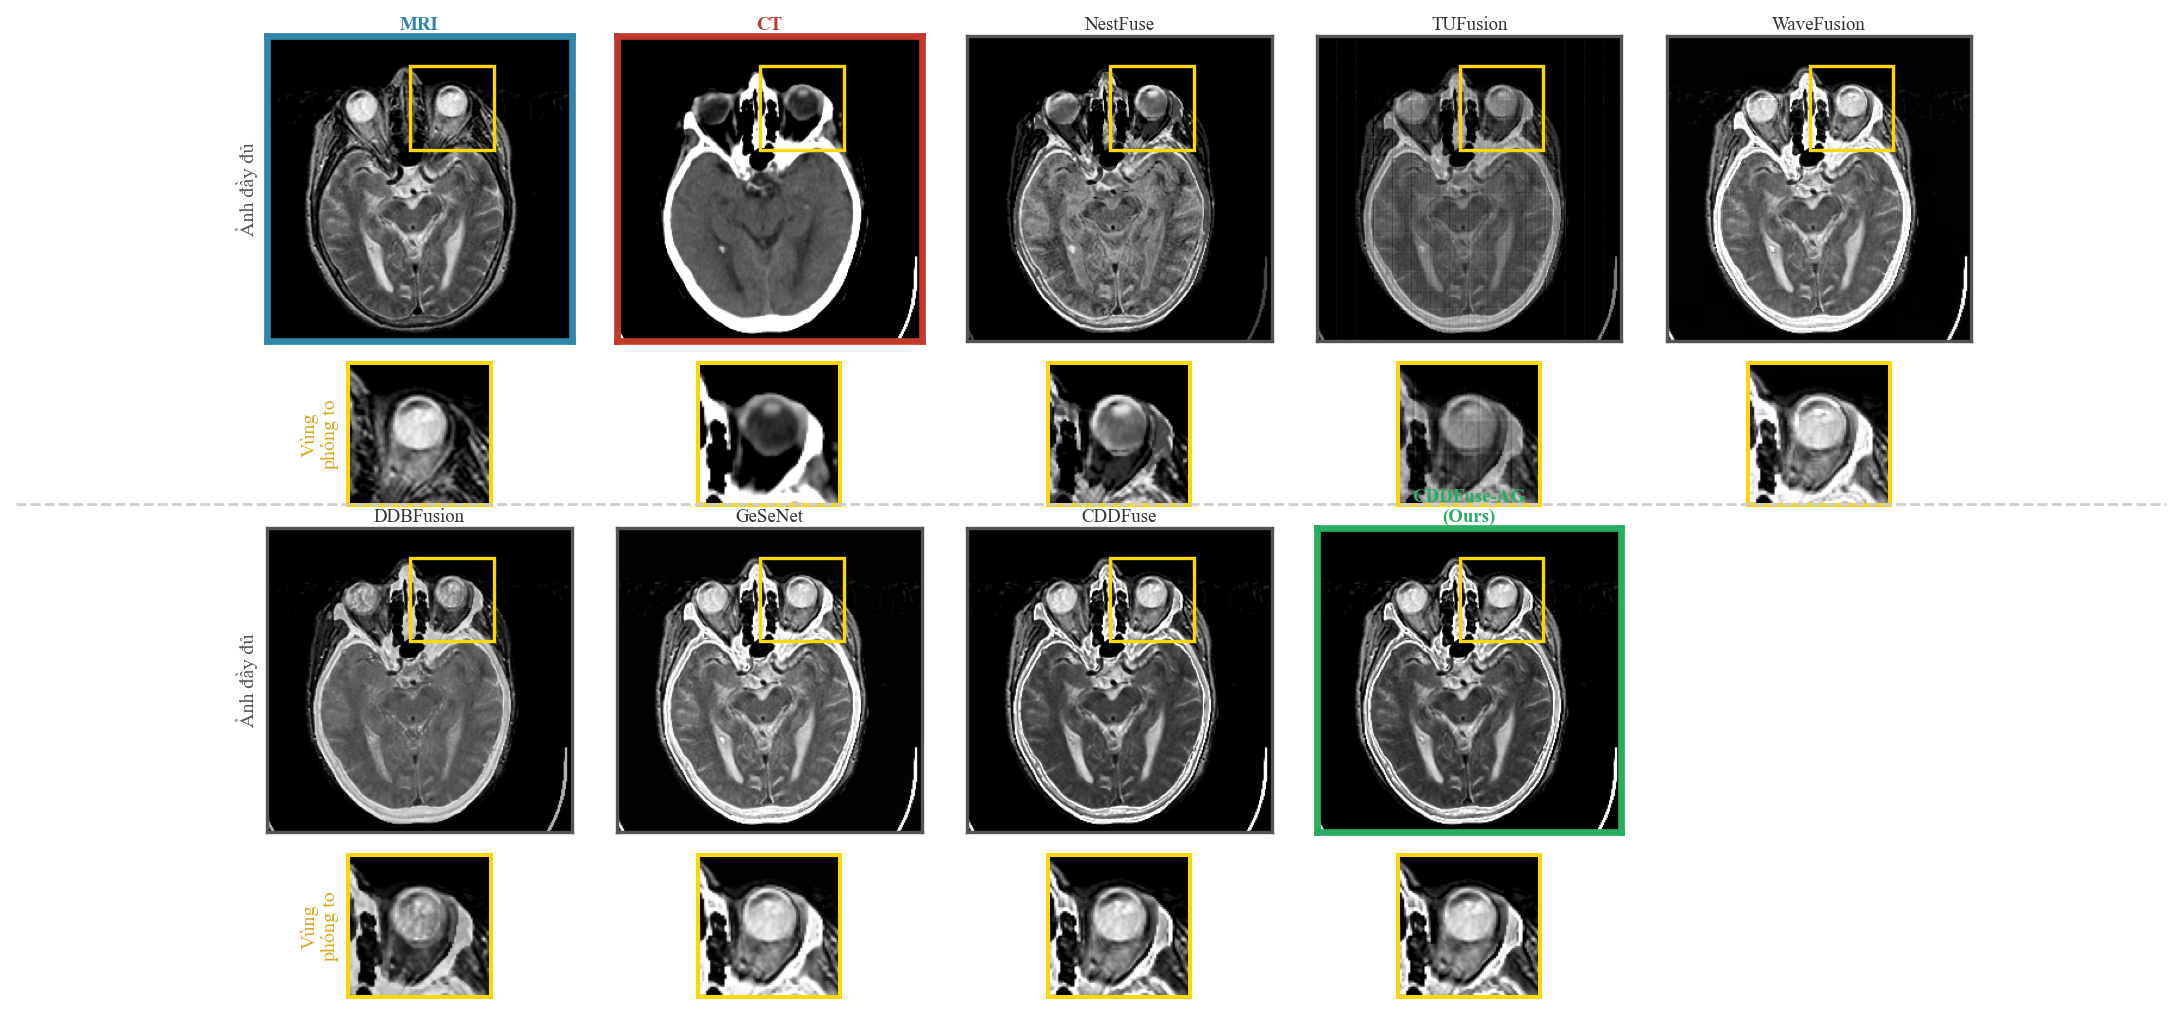
\includegraphics[width=\columnwidth]{fig_visual_comparison.png}
  \caption{So sánh trực quan MRI-CT. Hàng trên: ảnh đầy đủ;
  hàng dưới: phóng to vùng hốc mắt phải. CDDFuse-AG (khung xanh) giữ
  cạnh xương sắc nét nhất.}
  \label{fig:visual-ct}
\end{figure}

% ============================================================
\section{Thảo luận}
\label{sec:discussion}

\subsection{Phát hiện Modality-Specificity}

Kết quả Stage 3 cho thấy không có quy tắc tổng hợp đơn lẻ nào tối ưu cho mọi
modality: CDDFuse-AG tốt nhất trên CT-MRI, CDDFuse (Sum) dẫn trên SPECT-MRI.
Lý giải:
\begin{itemize}\itemsep1pt
  \item \textbf{CT-MRI}: Cạnh xương (CT) và mô mềm (MRI) không chồng lấp, SML
        phân biệt chính xác vùng nào ưu tiên modality nào, WAvg cân bằng toàn
        cục hiệu quả cho Base.
  \item \textbf{SPECT-MRI}: SPECT có đặc trưng thưa thớt, ít thông tin chi tiết
        -- mọi quy tắc lựa chọn phức tạp đều có xu hướng tạo artifact; Sum đơn
        giản an toàn hơn.
\end{itemize}

Kết quả gợi ý \textbf{modality-aware routing}: chọn fusion rule tự động dựa trên
đặc tính phân phối của từng cặp modality đầu vào, thay vì dùng một chiến lược
cố định.

\subsection{Tính giản dị và hiệu quả tham số}

WAvg với 1 scalar duy nhất dẫn đầu Stage 1 trên CT-MRI. Đây là minh chứng cho
nguyên tắc: khi Encoder đã pretrained tốt và phân rã đặc trưng ổn định, fusion
rule chỉ cần đúng hướng --- không cần phức tạp. LocalEntropy ($-0.990$ z avg)
thất bại vì entropy của feature-space không mang cùng ý nghĩa với entropy
pixel-space.

\subsection{Hạn chế}

SML không thích nghi với mức nhiễu khác nhau giữa modality, có thể ưu tiên nguồn
nhiễu cao thay vì nguồn có cạnh thực sự. Ngoài ra, toàn bộ đánh giá dựa trên chỉ
số tự động; nghiên cứu đọc ảnh lâm sàng (reader study) chưa được thực hiện.

% ============================================================
\section{Kết luận}
\label{sec:conclusion}

Bài báo đề xuất CDDFuse-AG, cải tiến CDDFuse thông qua thiết kế bất đối xứng:
WAvg cho nhánh Base và SML cho nhánh Detail. Chỉ với 4.161 tham số mới, mô hình
vượt CDDFuse trên CT-MRI ($+0.323$ z-score) và đạt z avg $+0.344$ --- cao nhất
trong nhóm 6 phương pháp so sánh trực tiếp. Phát hiện Modality-Specificity gợi
ý rằng fusion strategy nên được điều chỉnh theo đặc tính từng cặp modality, mở
hướng cho modality-aware routing và adaptive fusion trong tương lai.

% ============================================================
\bibliographystyle{IEEEtran}
\bibliography{../report_latex/bibliography}

\end{document}
